% -----------------------------------------------
% Appendix / backup slides. `\appendix` resets frame numbering and keeps these
% out of the main talk flow and the table of contents: they sit after the last
% "real" slide, so forward navigation during the talk never lands on them --
% you jump to them only if a question calls for it.
% -----------------------------------------------
\appendix

\begin{frame}{Appendix — TabPFN}
  \framesubtitle{Hyperparameters priors}
  \def\imgwidth{0.75}   % fraction of text width (0..1)
  \def\imgx{0cm}       % horizontal shift: + right, - left
  \def\imgy{-0.5cm}       % vertical shift:   + up,    - down
  \def\imglabel{Hyperparameters priors used to generate synthetic datasets.}      % caption shown below the image (leave empty for none)
  \begin{tikzpicture}[remember picture, overlay]
    \node[anchor=center, xshift=\imgx, yshift=\imgy] (img)
      at (current page.center)
      {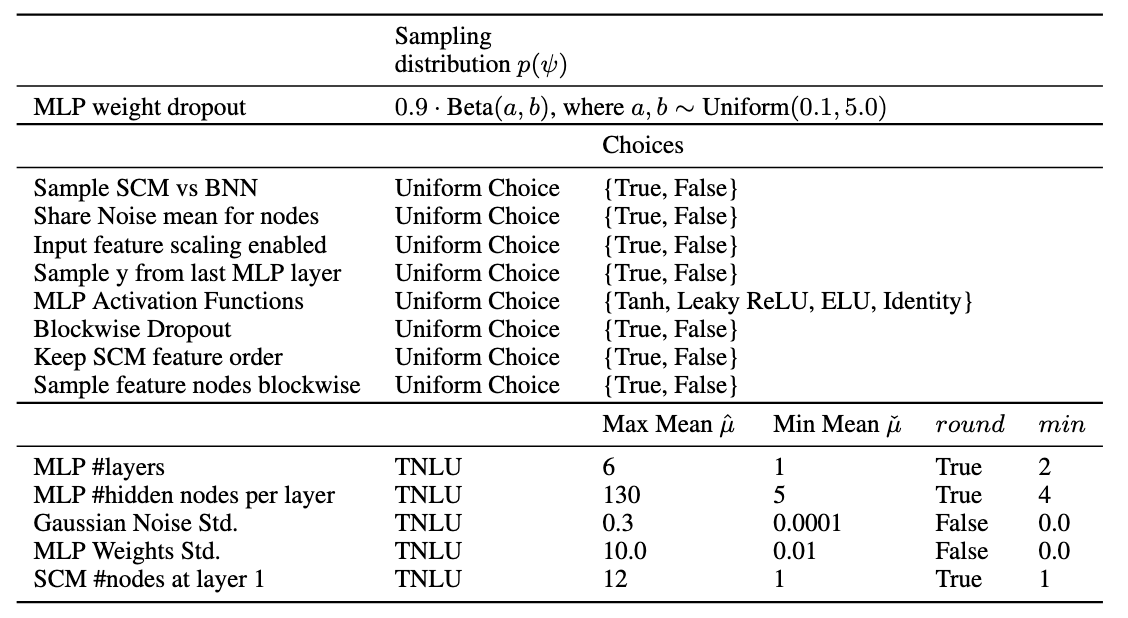
\includegraphics[width=\imgwidth\textwidth]{figures/tabpfn/prior-data/hp-priors.png}};
    \node[below=0.0cm of img] {\small\imglabel};
  \end{tikzpicture}
\end{frame}
